\chapter{THIẾT KẾ CƠ KHÍ}
    \section{Phân tích động học và động lực học xe}
        \subsection{Phân tích động lực học xe khi đi thẳng}
            \begin{figure}[H]
                \centering
                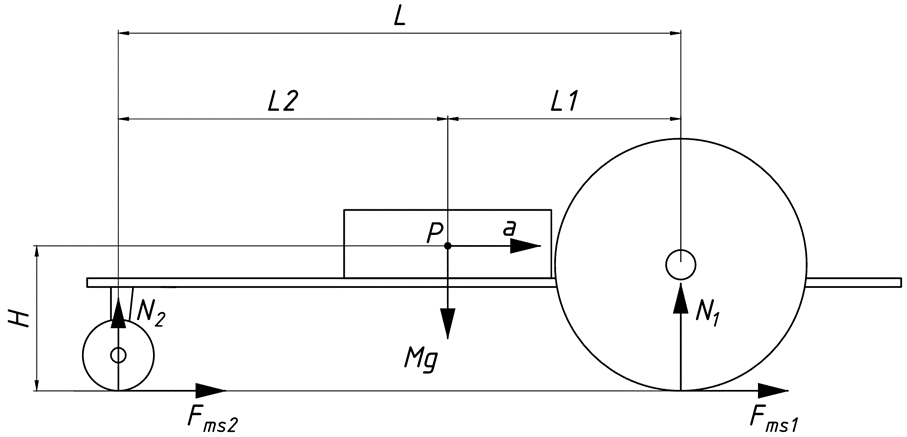
\includegraphics[width=1\textwidth]{pictures/chapter3/c3_p1_StraightAnalysis.png}
                \caption{Mô hình phân tích động lực học xe khi đi thẳng}
                \label{fig:3.1}
            \end{figure}
            \hspace*{0.6cm}Các thành phần lực:
            \begin{itemize}
                \item $N_1$ - Phản lực tại bánh dẫn động (N)
                \item $N_2$ - Phản lực tại bánh bị động trước (N)
                \item $N_3$ - Phản lực tại bánh bị động sau (N)
                \item $L = L_1 + L_2$ - Khoảng cách trục bánh trước và bánh sau (m)
                \item $H$ - Chiều cao từ trọng tâm xe đến mặt đất (m)
                \item $r$ - Bán kính bánh xe dẫn động (m)
                \item $M$ - Khối lượng của hệ (kg)
                \item $g = 9.8 \, m/s^2$ - Gia tốc trọng trường tại vị trí đang xét
                \item $a$ - Gia tốc của hệ ($m/s^2$)
            \end{itemize}
            \hspace*{0.6cm}Phương trình cân bằng lực:
            \begin{equation}
                \begin{cases}
                    \sum F_x = 0 \Rightarrow 2F_{ms1} + F_{ms2} = Ma \\
                    \sum F_y = 0 \Rightarrow 2N_1 + N_2 = Mg \\
                    \sum M_{z/c} = 0 \Rightarrow 2N_2L_1 - 2F_{ms2}H - 2F_{ms1}H - 2N_1L_1 - 2F_{ms1}H = 0
                \end{cases}
                \label{eq:3-1}
            \end{equation}
            \begin{equation}
                \Rightarrow
                \begin{cases}
                    2F_{ms1} + F_{ms2} = Ma  \\[0.2cm]
                    N_1 = \dfrac{MgL_2}{2L} - \dfrac{MaH}{2L} \\[0.2cm]
                    N_2 = \dfrac{MgL_1}{2L} + \dfrac{MaH}{2L}
                \end{cases}
                \label{eq:3-2}
            \end{equation}
        \subsection{Điều kiện để bánh xe luôn bám mặt đường}
            \hspace*{0.6cm}Để bánh xe luôn bám mặt đường thì phản lực tại điểm tiếp xúc giữa bánh xe và mặt đường luôn lớn hơn không khi đó:
            \begin{equation}
                \begin{cases}
                    N_1 = \dfrac{MgL_2}{2L} - \dfrac{MaH}{2L} \\[0.3cm]
                    N_2 = \dfrac{MgL_1}{2L} + \dfrac{MaH}{2L}
                \end{cases}
                \label{eq:3-3}
            \end{equation}
            \begin{equation}
                \Rightarrow
                L_{2}g > aH
                \label{eq:3-4}
            \end{equation}
        \subsection{Điều kiện để xe không bị lật khi vào cua}
            \begin{figure}[H]
                \centering
                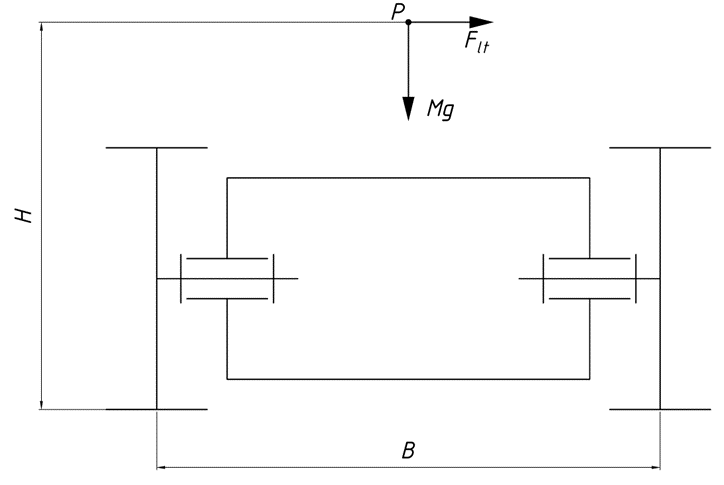
\includegraphics[width=0.6\textwidth]{pictures/chapter3/c3_p2_TurningAnalysis.png}
                \caption{Mô hình phân tích động lực học xe khi vào cua không lật}
                \label{fig:3.2}
            \end{figure}
            \hspace*{0.6cm}Để xe không lật thì momen do lực li tâm gây ra không lớn hơn moment do trọng lực gây ra:
            \begin{align}
                F_{lt}H &\leq P \times \dfrac{B}{2} \label{eq:3-5a} \\
                \Rightarrow \dfrac{B}{H} &\geq \dfrac{2F_{lt}}{Mg} \Rightarrow \dfrac{B}{H} \geq \dfrac{2Mv_{max}^2}{RMg} \label{eq:3-5b} \\ 
                \Rightarrow \dfrac{B}{H} &\geq \dfrac{2 \times 0.5^2}{0.5 \times 9.8} = 0.102 \label{eq:3-5c}
            \end{align}
            \hspace*{0.6cm}Trong đó: $v_{max} = 0.5$ m/s; $R = \rho_{min} = 0.5$ m; $g = 9.8$ m/s$^2$.
        \subsection{Điều kiện để xe không trượt khi vào cua}
            \begin{figure}[H]
                \centering
                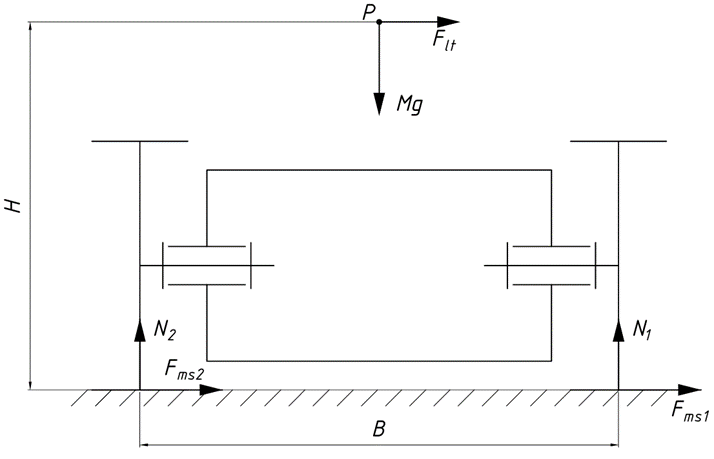
\includegraphics[width=0.6\textwidth]{pictures/chapter3/c3_p3_TurningAnalysis2.png}
                \caption{Mô hình phân tích động lực học xe khi vào cua không trượt}
                \label{fig:3.3}
            \end{figure}
            \hspace*{0.6cm}Để xe không trượt khi vào cua thì lực hướng tâm, trong trường hợp này là tổng lực ma sát tác dụng lên xe lớn hơn lực li tâm:
            \begin{align}
                \sum F_{ms} &\geq Ma_n \label{eq:3-12} \\
                \Rightarrow \mu Mg &\geq \dfrac{Mv_{max}^2}{r} \label{eq:3-13} \\
                \Rightarrow v_{max} &\leq \sqrt{\mu gR} \label{eq:3-14}
            \end{align}
            \hspace*{0.6cm}Tóm lại ta có các ràng buộc từ công thức (\ref{eq:3-12}), (\ref{eq:3-13}) và (\ref{eq:3-14}):
            \begin{equation}
                \begin{cases}
                    &L_2 g > aH \\
                    &\dfrac{B}{H} > 0.102 \\
                    &v_{\text{max}} \geq \sqrt{\mu g R}
                \end{cases}
                \label{eq:3-15}
            \end{equation}
            \hspace*{0.6cm}Trong đó: $v_{\text{max}} = 0.5 \,\mathrm{m/s}; \, R = \rho_{\text{mix}} = 500 \,\mathrm{mm} = 0.5 \,\mathrm{m}; \, g = 9.8 \,\mathrm{m/s^2}; \, \mu = 0.6$.\\
            \hspace*{0.6cm}\textbf{Chọn sơ bộ:}\\
            \begin{itemize}
                \item Chọn khoảng cách giữa 2 động cơ cũng n    hư tiện đi dây, lúc này khoảng cách tâm hai bánh xe dẫn động: chọn $B = 220 \,(\mathrm{mm})$.
                \item Trọng tâm xe càng thấp xe càng ổn định nhưng phụ thuộc vào cách bố trí cách thành phần khác nên khoảng cách trọng tâm xe tới sàn sẽ được thay đổi liên tục trong quá trình thiết kế. chọn $H = 63.6 \,(\mathrm{mm})$.
                \item -	Khoảng cách tâm dãy cảm biến đến trục bánh dẫn động càng nhỏ thì xe càng ổn định, tuy nhiên khoảng cách này phải lớn hơn khoảng cách xe di chuyển được sau một lần lấy mẫu và phù hợp với cách bố trí các thành phần khác, sau khi mô phỏng qua matlab thì nhóm chọn $d = 72 \,(\mathrm{mm})$.
            \end{itemize}
            \hspace*{0.6cm}Tóm lại:
            \begin{equation*}
                B = 220 \,\mathrm{mm}; \, H = 63.6 \,\mathrm{mm}; \, L = 190 \,\mathrm{mm}; \, L_1 = 89 \,\mathrm{mm}; \, L_2 = 101 \,\mathrm{mm}
            \end{equation*}
            \hspace*{0.6cm}Thay số vào (\ref{eq:3-15}) ta được
            \begin{equation*}
                \begin{cases}
                \dfrac{0.101 \times 9.8 > 0.5 \times 0.0636}{0.22} \\
                \dfrac{0.0636}{0.0636} > 0.102 \\
                0.5 \leq \sqrt{0.6 \times 9.8 \times 0.5}
                \end{cases}
                \Leftrightarrow
                \begin{cases}
                0.9898 > 0.0318 \\
                3.459 > 0.102 \\
                0.5 \leq 1.715
                \end{cases}
            \end{equation*}           
    \section{Tính toán và chọn động cơ}
        \hspace*{0.6cm}\textbf{Thông số đầu vào}:
        \begin{itemize}
            \item $v_{\text{max}} = 0.5 \,\mathrm{m/s}$ - vận tốc tối đa mong muốn.
            \item $r = 85 \,\mathrm{mm}$ - bán kính bánh xe chủ động.
            \item $t = 1 \,\mathrm{s}$ - thời gian xe tăng tốc từ 0 đến 0.5 m/s.
        \end{itemize}
        \hspace*{0.6cm}Gia tốc của xe
        \begin{equation*}
            a = \dfrac{0.5 - 0}{1} = 0.5 \,\mathrm{m/s^2}
        \end{equation*}
        \hspace{0.6cm}Vận tốc góc của bánh xe chủ động
        \begin{equation*}
            \omega = \dfrac{v_{\text{max}}}{r} = \dfrac{0.5}{0.085/2} = 11.765 \,\mathrm{rad/s}
        \end{equation*}
        \hspace*{0.6cm}Gia tốc góc
        \begin{equation*}
            \gamma = \frac{a}{r} = \dfrac{0.5}{0.085/2} = 11.765 \,\mathrm{rad/s^2}
        \end{equation*}
        \hspace*{0.6cm}Xét tại vị trí một bánh xe, ta có mô hình phân tích lực của hệ\\
        %figure
        \begin{figure}[H]
            \centering
            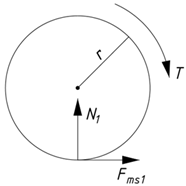
\includegraphics[width=0.3\textwidth]{pictures/chapter3/banhxe.png}
            \caption{Mô hình phân tích tích lực bánh xe chủ động}
            \label{phantich_banhxe}
        \end{figure}
        \hspace*{0.6cm}Giả sử bánh xe dạng tròn, đồng chất, có moment quán tính như sau
        \begin{equation}
            I = \dfrac{1}{2}mr^2
            \label{eq:3-16}
        \end{equation}
        \hspace*{0.6cm}Phương trình cân bằng moment tại tâm bánh xe dẫn động
        \begin{equation}
            \tau - F_{\text{ms1}} r = I \gamma
            \label{eq:3-17}
        \end{equation}
        Thế (\ref{eq:3-16}) vào (\ref{eq:3-17}) ta được
        \begin{align*}
            \tau - F_{\text{ms1}} r &= \frac{1}{2}mr^2\gamma \\
            &= \frac{1}{2}mr^2\gamma + F_{\text{ms1}}r \\
            &= \frac{1}{2}mr^2\gamma + \mu_t\left(\frac{1}{2}M + m\right)gr \\
            &= \frac{1}{2} \times 0.06 \times \left(\frac{0.085}{2}\right)^2 \times 15.38 + 0.1 \times \left(\frac{1}{2} \times 2.2 + 0.06\right) \times 9.8 \times \frac{0.085}{2} \\
            &= 0.05 \,\text{Nm}
        \end{align*}
        \hspace*{0.6cm}Trong đó
        \begin{itemize}
            \item $I$: momen quán tính ($\mathrm{kg.m^2}$).
            \item $r = 0.0425 \,\mathrm{m}$ - bán kính bánh xe chủ động.
            \item $m = 0.06 \,\mathrm{kg}$ - khối lượng bánh xe chủ động.
            \item $\tau$: momen xoắn để bánh xe quay.
            \item $\gamma = 15.38 \,\mathrm{rad/s^2}$.
            \item $M = 2.2 \,\mathrm{kg}$.
            \item $\mu = 0.1$: hệ số ma sát lăn.
            \item $K = 2.5$: hệ số an toàn.
        \end{itemize}
        \hspace*{0.6cm}Số vòng quay động cơ
        \begin{equation*}
            n_{\text{motor}} = \dfrac{60v_{\text{max}}}{2\pi r} = \dfrac{60 \times 0.5}{2 \pi \dfrac{0.085}{2}} = 112.345 \,\mathrm{rpm}
        \end{equation*}
        \hspace*{0.6cm}Công suất cần thiết của động cơ
        \begin{align*}
            P = \tau \omega = K \times \dfrac{\tau \times 2 \pi \times n_{\text{motor}}}{60} = 2.5 \times \dfrac{0.05 \times 2 \pi \times 112.345}{60} = 0.735 \,\mathrm{W}
        \end{align*}
        \hspace*{0.6cm}Dựa theo công suất và số vòng quay tính được, ta chọn động cơ JGB37-520 ($\omega = 333 \,\mathrm{rpm}, \, P = 9 \,\mathrm{W}$).
        \begin{figure}[H]
            \centering
            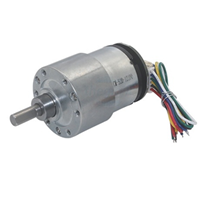
\includegraphics[width=0.4\textwidth]{pictures/chapter3/motor.png}
            \caption{Động cơ JGB37-520 12VDC 333 RPM}
            \label{dc}
        \end{figure}
        \begin{table}[h]
            \centering
            \caption{Bảng thông số kỹ thuật động cơ JGB37-520 (333 rpm)}
            \begin{tabular}{|p{5cm}|c|c|}
            \hline
            \textbf{Thông số} & \textbf{Giá trị} & \textbf{Đơn vị} \\
            \hline
            Đường kính trục động cơ & 6 & mm \\
            \hline
            Đường kính động cơ & 37 & mm \\
            \hline
            Công suất & 9 & W \\
            \hline
            Tỷ số truyền & 30:1 & - \\
            \hline
            Tốc độ tối đa & 333 & rpm \\
            \hline
            Moment kéo tối đa & 5 & kg.cm \\
            \hline
            \begin{tabular}[c]{@{}c@{}}Độ phân giải Encoder (2\\kênh A,B)\end{tabular} & 660 & xung/vòng \\
            \hline
            \end{tabular}
        \end{table}
    \section{Thiết kế sơ bộ gá động cơ}
        \begin{figure}[H]
            \centering
            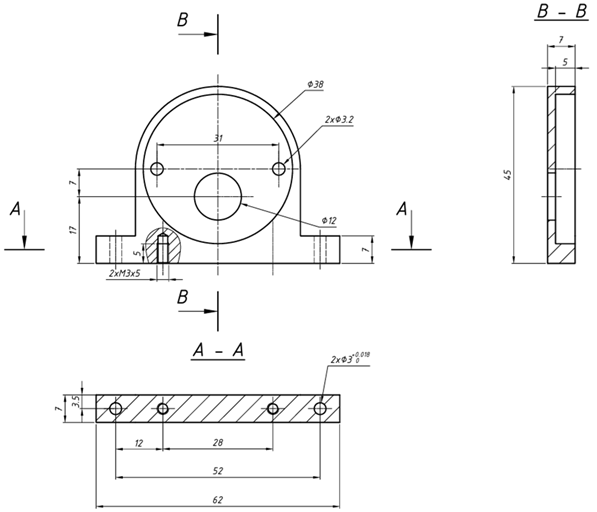
\includegraphics[width=0.8\textwidth]{pictures/chapter3/ga_dc.png}
            \caption{Thiết kế sơ bộ đồ gá động cơ}
            \label{ga_dc}
        \end{figure}
    \section{Mô hình 3D}
        \hspace*{0.6cm}Dựa theo mô hình 3D thiết kế ta xác định được các kích thước cuối cùng cho bản vẽ thiết kế như sau
         \begin{table}[h!]
            \centering
            \caption{Bảng thông số kỹ thuật của xe}
            \begin{tabular}{|l|c|c|}
                \hline
                \textbf{Thông số} & \textbf{Giá trị} & \textbf{Đơn vị} \\ \hline
                Kích thước xe (LxBxH) & 286.5$\times$252$\times$113 & mm \\ \hline
                Khoảng cách tâm dãy cảm biến đến trục bánh chủ động & 72 & mm \\ \hline
                Khoảng cách tâm 2 bánh chủ động & 220 & mm \\ \hline
                Khoảng cách tâm bánh bị động và chủ động & 190 & mm \\ \hline
            \end{tabular}
        \end{table}
        \begin{figure}[H]
            \centering
            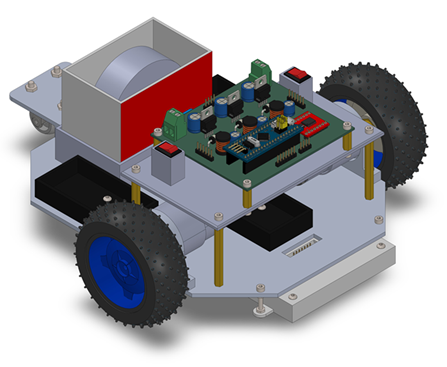
\includegraphics[width=0.7\textwidth]{pictures/chapter3/3d.png}
            \caption{Thiết kế 3D của xe}
            \label{3d}
        \end{figure}
        \hspace*{0.6cm}\textbf{Kết luận:} điều kiện được thỏa mãn cho nên mô hình thiết kế đám ứng được các yêu cầu về động học và động lực học giúp cho điều khiển và lập trình được dễ dàng hơn.


